\documentclass{article}[12pt]

\usepackage[utf8]{inputenc}
\usepackage{amsfonts,amssymb,amsmath,subfigure}
\usepackage[pdftex]{graphicx}
\usepackage{epstopdf}
\usepackage{vmargin}
\usepackage{comment}
\usepackage{tikz,multicol}

\usepackage{algorithm}
\usepackage[noend]{algpseudocode}
\usepackage{tcolorbox}

\newtcolorbox{mybox}[3][]
{
  colframe = #2!25,
  colback  = #2!10,
  coltitle = #2!20!black,  
  title    = {#3},
  #1,
}


\newcommand*\Let[2]{\State #1 $\gets$ #2}
\algrenewcommand\algorithmicrequire{\textbf{Precondition:}}
\algrenewcommand\algorithmicensure{\textbf{Postcondition:}}




\excludecomment{solution}
%\includecomment{solution}

\title{IF111 - Algorithmes et structures de données\\EI3 - Structures de données et arbres de recherche}
\date{\texttt{rfosse@labri.fr}}
\author{Rohan Fossé}
\begin{document}



\maketitle{}


\section*{Recherche dans un ABR}
\begin{enumerate}
    \item Écrire une fonction qui retourne $true$ si l’ABR qui lui est passé en paramètre
est une feuille.
    \item  Écrire une fonction récursive qui affiche l’ABR qui lui est passé en paramètre, par ordre croissant des valeurs.
    \item Écrire une fonction récursive qui affiche l’ABR qui lui est passé en paramètre, par ordre décroissant des valeurs.
    \item Écrire une fonction qui retourne la hauteur de l’ABR qui lui est passé en
paramètre.
\item Écrire une fonction qui retourne le nombre de nœuds de l’ABR qui lui est
passé en paramètre.
\end{enumerate}

\begin{figure}[hbtp] 
  \centering
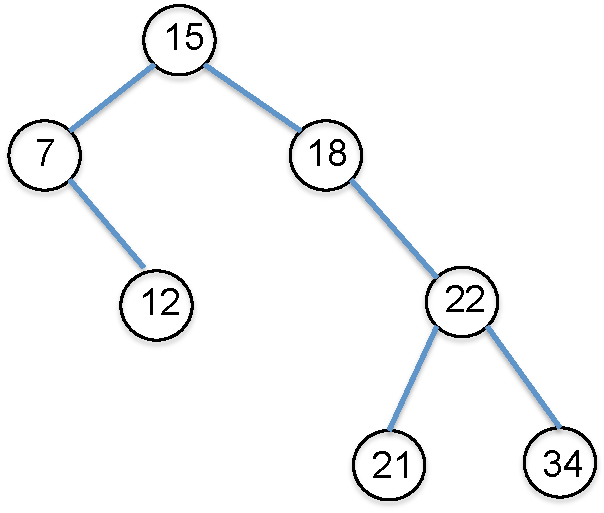
\includegraphics[scale =0.5] {ABR.pdf}\label{fig:abr} \caption{Arbre binaire de recherche}
\end{figure}

\section*{Suppression dans un arbre binaire de recherche}
Soit l’arbre binaire de recherche donné dans la figure 1
\begin{enumerate}
    \item Dessiner l’arbre après la suppression du noeud 18.
    \item  L’opération suppression est-elle ”commutative” au sens où la suppression de x puis de y dans un arbre binaire de recherche produit le même arbre que la suppression de y puis
de x.\\
Si oui dire pourquoi, sinon donner un contre exemple.
\end{enumerate}




\section*{Algorithme de Dijkstra}
On considère maintenant des graphes pondérés. Appliquer l'algorithme de Dijkstra au graphe dans la Figure \ref{fig:grapheDijkstra} pour calculer la plus courte distance de $B$ à $D$.

\begin{figure}[h!] 
  \centering
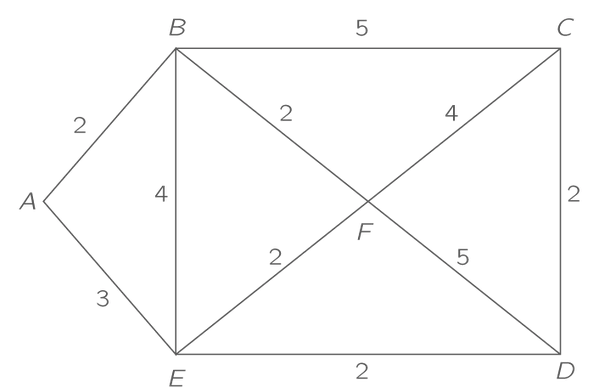
\includegraphics[scale =0.4]{Djikstra.png}
\caption{Graphe pour Dijkstra.} \label{fig:grapheDijkstra}
\end{figure}

\section*{Récursivité sur les arbres}
\begin{enumerate}
\item Dessiner l'arborescence binaire ayant 10 noeuds \{0, 1, 2, ..., 9\}, telle que le parcours infixe et le parcours postfixe de cette arborescence produisent respectivement les suites suivantes : 9, 3, 1, 0, 4, 2, 6, 7, 8, 5 (infixe) et 9, 1, 4, 0, 3, 6, 7, 5, 8, 2 (postfixe). Dire quel est le raisonnement utilisé pour arriver à la solution.\\ Dire quelle est la hauteur du noeud 1 et 2 dans l'arborescence dessinée et quelle est la hauteur de l'arborescence elle même. \\

\end{enumerate}

\section*{Coloration de graphes}

\begin{figure}[h!]
    \centering
    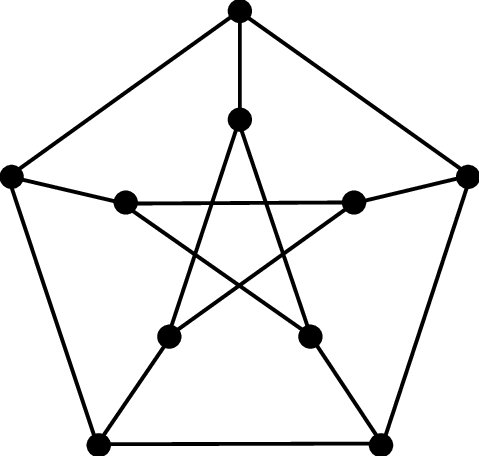
\includegraphics[scale=0.3]{Petersen.png}
    \caption{Graphe de Petersen}
    \label{fig:petersen}
\end{figure}

On cherche à colorier le graphe de la figure \ref{fig:petersen} en utilisant des entiers positifs de façon telle que deux sommets voisins ont des couleurs dont la différence, en valeur absolue, est au moins égale à trois.


\section*{La bibliothèque}

Sept élèves, désignés par A,B,C,D,E,F et G se sont rendus à la bibliothèque aujourd'hui. Le tableau suivant précise "qui a rencontré qui" (la bibliothèque étant petite, deux élèves présents au même moment se rencontrent nécessairement…). 

\begin{table}[h!]
\begin{tabular}{|c|c|c|l|l|l|l|l|}
\hline
\textbf{élève}       & \textbf{A} & \textbf{B} & \textbf{C} & \textbf{D} & \textbf{E}  & \textbf{F} & \textbf{G} \\ \hline
\textbf{a rencontré} & D,E        & D,E,F,G    & E,G        & A,B,E      & A,B,C,D,F,G & B,E,G      & B,C,E,F    \\ \hline
\end{tabular}
\end{table}

De combien de places assises doit disposer la bibliothèque pour que chacun ait pu travailler correctement au cours de cette journée ?

\section*{Graphes complets}

Tout graphe contenant un triangle ($K_3$) ne peut être colorié en moins de trois couleurs.

\begin{enumerate}
    \item Construire un graphe sans triangle qui nécessite également trois couleurs.
    \item Comment construire un graphe sans $K_4$ nécessitant 4 couleurs ?
    \item un graphe sans $K_5$ nécessitant 5 couleurs ?
\end{enumerate}

\section*{Les dominos}

On considère des dominos dont les faces sont numérotées 1, 2, 3, 4 ou 5.

\begin{enumerate}
    \item En excluant les dominos doubles, de combien de dominos dispose-t-on ?
    \item Montrez que l’on peut arranger ces dominos de façon à former une boucle fermée (en utilisant la règle habituelle de contact entre les dominos).
    \item Pourquoi n’est-il pas nécessaire de considérer les dominos doubles ?
    \item Si l’on prend maintenant des dominos dont les faces sont numérotées de 1 à n, est-il possible de les arranger de façon à former une boucle fermée ?
\end{enumerate}

\section*{Graphes Eulériens}

Soit G un graphe non Eulérien. Est-il toujours possible de rendre G Eulérien en lui rajoutant un sommet et quelques arêtes ?


Pour qu’un graphe soit eulérien, il faut et il suffit que tous ses sommets soient de degré pair. Si un graphe contient k sommets impairs, il est possible de rajouter un nouveau sommet x, relié à ces k sommets. Dans le graphe obtenu, les k sommets considérés sont devenus pairs… Cependant, le degré de x étant k, le graphe n’est toujours pas eulérien si k était impair…

Remarquons qu’il est possible de rajouter des arêtes entre les sommets de degré impair dans le graphe d’origine… Mais l’ajout d’une telle arête, entre deux sommets impairs a et b par exemple, fait que le nombre de sommets impairs devient k-2, qui a la même parité que k…

La réponse est donc : ce n’est possible que si le nombre de sommets impairs est pair…


\end{document}